\documentclass{beamer}

\usepackage{tikz}
\usepackage{listings}
\usetikzlibrary{automata,positioning}
\usepackage{attrib}
\lstset{
basicstyle=\footnotesize \ttfamily,
language=Promela,
numbers=left,
xleftmargin=2em,
framexleftmargin=1.5em
}

\title{Model Checking}
\subtitle{Modeling concurrent systems and specification of correctness properties}
\author{Lukas Hofmaier \texttt{lukas.hofmaier@hsr.ch}}
\date{June 19, 2013 \\ Progam Analysis and Transformation Seminar FS13}

\begin{document}
\maketitle
\begin{frame}
  \frametitle{Outline}
  \tableofcontents
\end{frame}

\section{Model Checking}

\begin{frame}
  \frametitle{What's all about?}
  Does a behavioral model $S$ satisfy a defined property $P$?
  \[
  S \models P
  \]
  \begin{description}
  \item[S] Model written in Promela, describes the behavior of a system
  \item[$\models$] Satisfaction relation
  \item[P] Property to vefify, written in LTL notation
  \end{description}
\end{frame}

\begin{frame}
  \frametitle{Why Model Checking}
  \begin{description}
  \item[Peer review] Code is analyzed statically. Difficult to detect errors caused by concurrency.
  \item[Testing] Code is compiled and executed. Can expose error. Cannot proof absence of errors.
  \end{description}\
Model checking checks 100\% of all possible paths.
\end{frame}

\section{Modeling Concurrent Systems}

\begin{frame}
  \frametitle{  Defining $S$ in $S \models P$}

  \begin{itemize}
  \item   Spin checks verification models.
  \item The specification language that it accepts is called Promela.
  \item Emphasis of Promela is on modeling of process synchronization.
  \end{itemize}
\end{frame}

\subsection{Interleaving}

\begin{frame}
  \frametitle{Interleaving}
  \begin{itemize}
  \item Program statements are interlocked.
  \item Interleaving is a enumeration of all possible state sequences.
  \end{itemize}
\end{frame}

\begin{frame}[fragile]
  \frametitle{State diagram representation}
  \begin{columns}

    \begin{column}{.5\textwidth}
      \begin{figure}
        \centering
\begin{lstlisting}
byte x=0;

active proctype A(){
       byte tempA = x + 2;
       x = tempA;
}
\end{lstlisting}
      \end{figure}
    \end{column}

    \begin{column}{.5\textwidth}
      
      \begin{figure}
        \centering
        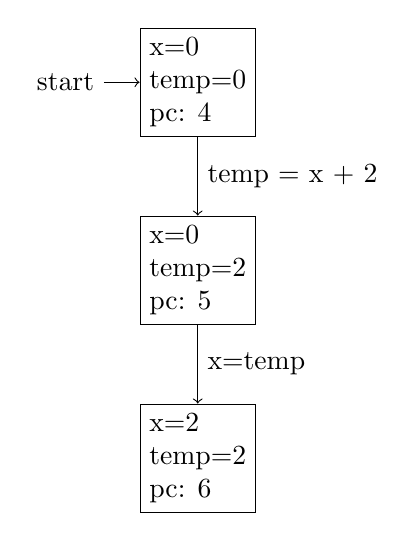
\begin{tikzpicture}[auto]
          \node[state, initial, rectangle, align=left](s1){x=0\\ temp=0\\pc: 4};
          \node[state, rectangle, align=left, below =of s1](s2){x=0\\temp=2\\pc: 5};
          \node[state, rectangle, align=left, below =of s2](s3){x=2\\temp=2\\pc: 6};
          \path[->](s1) edge node {temp = x + 2}(s2);
          \path[->](s2) edge node {x=temp}(s3);
        \end{tikzpicture}   
      \end{figure} 
    \end{column}    
  \end{columns}

\end{frame}

\begin{frame}[fragile]
  \frametitle{System with two active processes}
  \lstinputlisting{interleavingproc.pml}
\end{frame}

\begin{frame}[fragile]
  \frametitle{Interleaved perspective}
  \begin{figure}
    \centering
    
\scalebox{0.8}{
   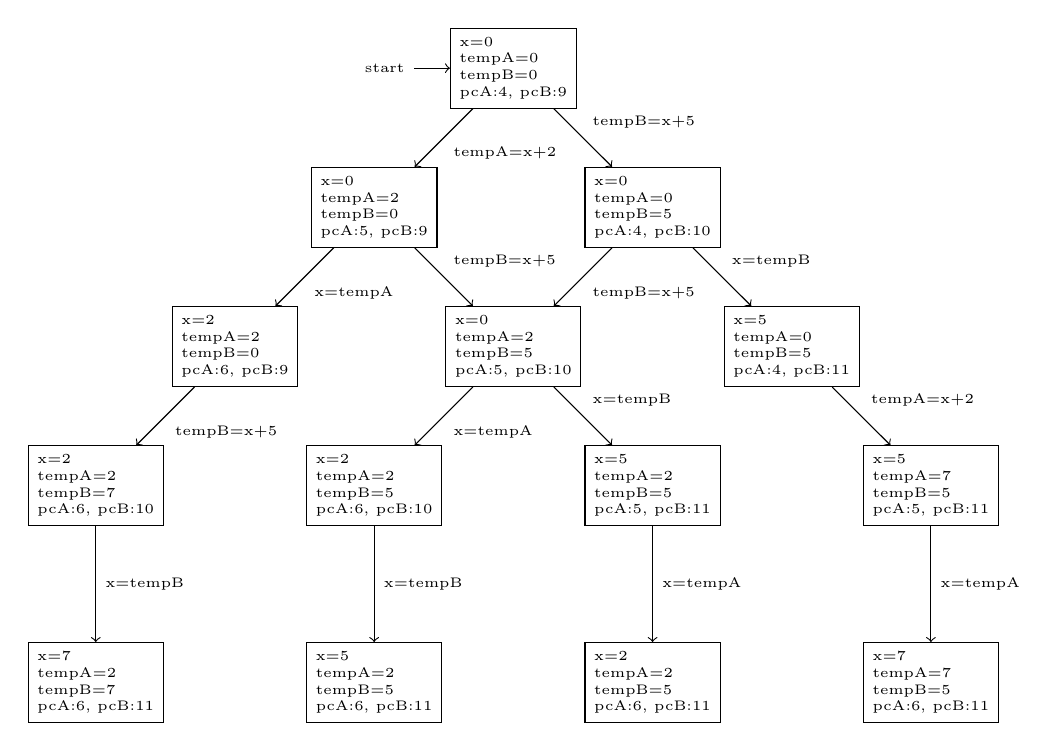
\begin{tikzpicture}[node distance=2.5cm, on grid, auto]
\tikzstyle{every node}=[font=\tiny]
   \node[state, initial, rectangle, align=left](s1){x=0\\tempA=0\\tempB=0\\pcA:4, pcB:9};
   \node[state, rectangle, align=left](s2) [below left=of s1]{x=0\\tempA=2\\tempB=0\\pcA:5, pcB:9};
   \node[state, rectangle, align=left](s3)[below left=of s2]{x=2\\tempA=2\\tempB=0\\pcA:6, pcB:9};
  \node[state, rectangle, align=left](s4)[below left=of s3]{x=2\\tempA=2\\tempB=7\\pcA:6, pcB:10};
\node[state, rectangle, align=left](s5)[below =of s4]{x=7\\tempA=2\\tempB=7\\pcA:6, pcB:11};
\node[state, rectangle, align=left](s6)[below right=of s1]{x=0\\tempA=0\\tempB=5\\pcA:4, pcB:10};
\node[state, rectangle, align=left](s7)[below right=of s6]{x=5\\tempA=0\\tempB=5\\pcA:4, pcB:11};
\node[state, rectangle, align=left](s8)[below right=of s7]{x=5\\tempA=7\\tempB=5\\pcA:5, pcB:11};
\node[state, rectangle, align=left](s9)[below =of s8]{x=7\\tempA=7\\tempB=5\\pcA:6, pcB:11};
\node[state, rectangle, align=left](s10)[below right=of s2]{x=0\\tempA=2\\tempB=5\\pcA:5, pcB:10};
\node[state, rectangle, align=left](s11)[below left=of s10]{x=2\\tempA=2\\tempB=5\\pcA:6, pcB:10};
\node[state, rectangle, align=left](s12)[below right=of s10]{x=5\\tempA=2\\tempB=5\\pcA:5, pcB:11};
\node[state,rectangle, align=left](s13)[below =of s11]{x=5\\tempA=2\\tempB=5\\pcA:6, pcB:11};
\node[state, rectangle, align=left](s14)[below =of s12]{x=2\\tempA=2\\tempB=5\\pcA:6, pcB:11};
   \path[->](s1) edge node {tempA=x+2}(s2);
   \path[->](s2) edge node {x=tempA}(s3);
   \path[->](s3) edge node {tempB=x+5}(s4);
\path[->](s4) edge node {x=tempB}(s5);
\path[->](s1) edge node {tempB=x+5}(s6);
\path[->](s6) edge node {x=tempB}(s7);
\path[->](s7) edge node {tempA=x+2}(s8);
\path[->](s8) edge node {x=tempA}(s9);
\path[->](s2) edge node {tempB=x+5}(s10);
\path[->](s6) edge node {tempB=x+5}(s10);
\path[->](s10) edge node {x=tempA}(s11);
\path[->](s10) edge node {x=tempB}(s12);
\path[->](s11) edge node {x=tempB}(s13);
\path[->](s12) edge node {x=tempA}(s14);
\end{tikzpicture}
}
\end{figure}

\end{frame}

\subsection{Synchronization}

\begin{frame}
  \frametitle{Synchronization Motivation}
  \begin{quote}
    Race conditions are a real nemesis that should be eliminated at the root. For an application that deals with mutability, every single access to shared mutable state must be verified to be correct. Even if one of them is broken, the entire application is broken. This is a tall order for our concurrent app to fall apart, only a single line of code that deals with concurrency needs to take a wrong step. In fact, a significant number of concurrent Java apps are broken, and we simply don’t know it.

 \attrib{ - Venkat Subramaniam \cite{subra11} -}
  \end{quote} 

\end{frame}

\begin{frame}[fragile]
  \frametitle{Lock the critical section with a mutex}
  \begin{figure}
    \centering
    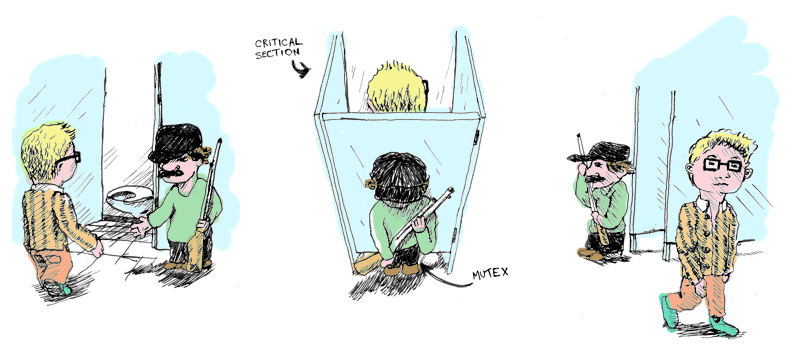
\includegraphics[scale=0.3]{mutex}
  \end{figure}
\begin{lstlisting}
#define acquire(mutex) atomic{mutex>0;mutex--;}
#define release(mutex) mutex++;
byte mutex=1
\end{lstlisting}

\end{frame}

\begin{frame}
  \frametitle{Locks are super tricky to use}
  \begin{figure}
    \centering
  
\includegraphics[scale=0.7]{dpsolved}
  \end{figure}
\end{frame}

\section{How to define correctness properties}

\begin{frame}
  \frametitle{Defining $P$ in $S \models P$}
  
  \begin{itemize}
    \item Linear Temporal Logic (LTL) is a formalism to express propositions in terms of time.
  \item  Linear Temporal Logic(LTL) is one way to define correctness properties in Spin.
  \item An formula of LTL is built from atomic propostions and from operators.
  \end{itemize}

\end{frame}

\subsection{Atomic propositions}


\begin{frame}
  \frametitle{Atomic Propositions}
  \begin{itemize}
  \item Declarative sentences. Can either be true or false.
  \item Evaluate to true or false
  \end{itemize}
  \begin{block}{Example}
    
  \end{block}
\end{frame}

\begin{frame}
  \frametitle{For Further Reading}

  \begin{thebibliography}{Subramaniam, 2011}

\bibitem{baier08}
Christel Baier Joost-Pieter Katoen,
Principles of Model Checking,
The MIT Press,
2008.

  \bibitem{subra11}
Venkat Subramaniam,
Programming Concurrency on the JVM: Mastering Synchronization, STM and Actors,
Pragmatic Bookshelf,
2011.

\end{thebibliography}
\end{frame}

\end{document}
%%% Local Variables: 
%%% mode: latex
%%% TeX-master: t
%%% End: 
